% vim: set spl=en:
\documentclass[smaller,t]{beamer}
\usepackage[utf8]{inputenc}
\usetheme{westlife}

\def\code#1{\structure{\texttt{#1}}}
\def\nadpis#1{\par\medskip\textbf{#1}}

\def\todo{{\color{red}\textbf{TODO}}}

\begin{document}
\makeatletter

\title{Virtualized Web Portals in EGI \\[\smallskipamount] Federated Cloud}
\date{MUSTweek, Brno, March 5--10}
\author[A. Křenek et al.]{Aleš Křenek, Radim Peša, Tomáš Raček, Vlastimil Holer, Daniel Kouřil, Ĺubomír Ontkoc}
\begin{frame}
\maketitle
\end{frame}

\begin{frame}{Security}

\nadpis{Motivation}
\begin{itemize}
\item Various views
\begin{itemize}
\item Users, service operator
\end{itemize}
\item Different requirements
\item We only show low-level bricks, always consider your needs
\end{itemize}

\nadpis{Security functions}
\begin{itemize}
\item Protection of information sent
\begin{itemize}
\item encryption and/or integrity protection
\end{itemize}
\item Authentication (of client and/or server)
\item Access control
\end{itemize}

\end{frame}


\begin{frame}{Security in Web Portals}
\begin{itemize}
\item Two possible levels to address security requirements
\begin{itemize}
\item Application itself (framework)
\item Web server (application container)
\end{itemize}
\item Well-established approaches to security for www
\item Protection of information 
\begin{itemize}
\item HTTP over TLS/SSL (https)
\end{itemize}
\item Authentication
\begin{itemize}
\item X.509 certificates, password-based
\item Single Sign-On
\end{itemize}
\item Access control
\begin{itemize}
\item Fine-grained (usually ad-hoc on application level)
\item Coarse grained (usable in container)
\item Based on authenticated identity or additional information
\end{itemize}
\end{itemize}
\end{frame}


\begin{frame}{Using TLS for Web Portals}
\nadpis{Enabling TLS}
\begin{itemize}
\item Server-based authentication and channel encryption
\item Client-side authentication also possible (out of scope for today)
\item Requirements:
\begin{itemize}
\item Digital certificate by a recognized CA
\item Automated process of getting the credentials
\end{itemize}
\end{itemize}

\nadpis{Certification Authority}
\begin{itemize}
\item Key cornerstone of traditional PKI
\item CAs available differ in many aspects and certificate types
\item IGTF provide a global trust platform for eScience but not accepted by
common applications
\item Let's encrypt CA available (if it matches the requirements)
\end{itemize}
\end{frame}


\begin{frame}{Security Assignment \#1}
\begin{itemize}
\item Deploy client to obtain X.509 server credentials from Let's encrypt CA
\item Enable TLS/SSL support in Apache
\end{itemize}

\begin{center}
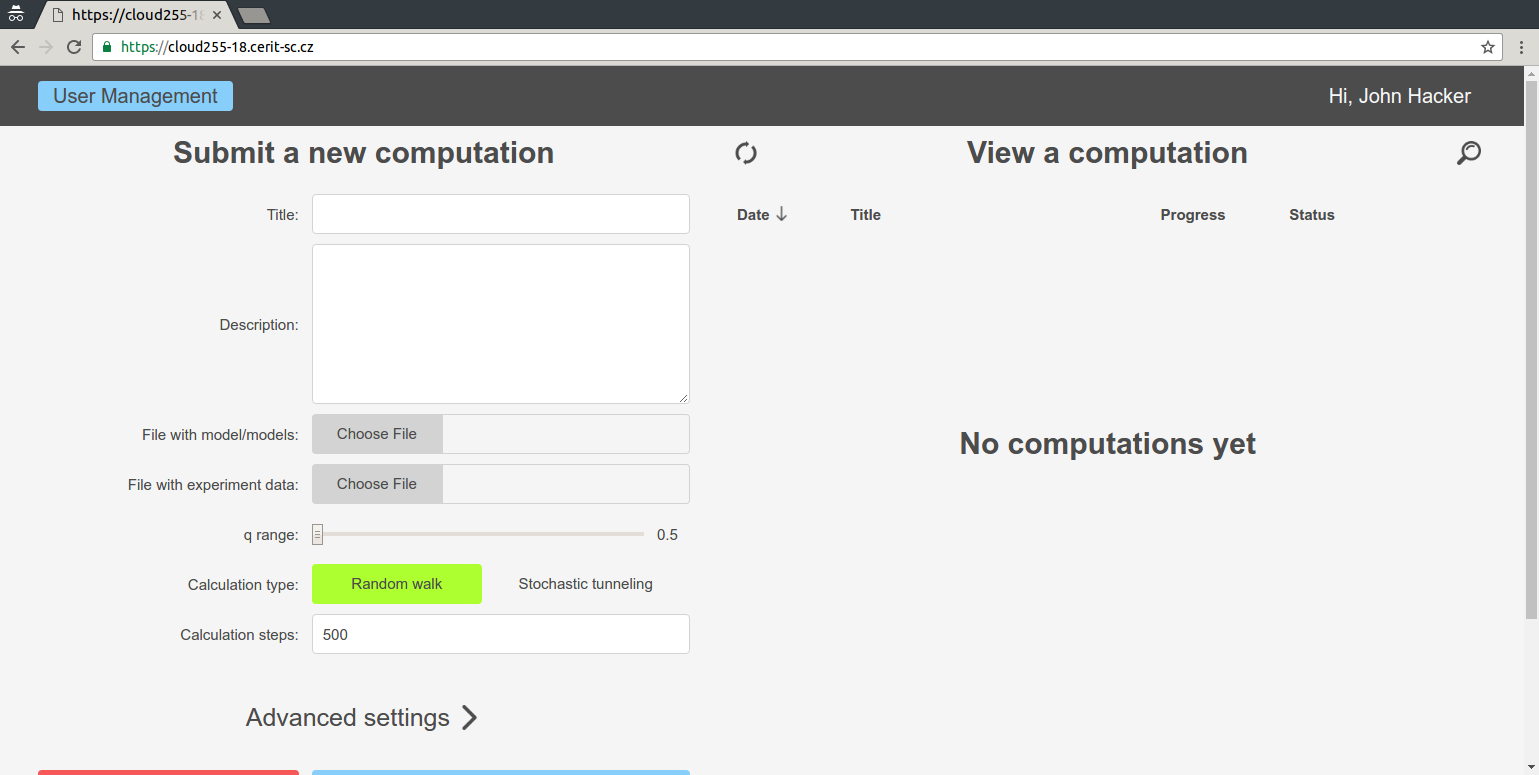
\includegraphics[width=.9\hsize]{https}
\end{center}
\end{frame}


\begin{frame}{Enable TLS in Portal}
\nadpis{Short Recap}
\begin{itemize}
\item Start from the configuration you finished yesterday
\item Continue to use your Docker container (\code{radimpesa/mustweek2017})
\item Weapons are available from
\code{git@github.com:ICS-MU/westlife-mustweek2017.git}
\item For slides see the \code{talks/} directory
\end{itemize}

\nadpis{Actions to perform}
\begin{itemize}
\item Start with two provided scripts
\begin{itemize}
\item \code{letsencrypt\_setup.sh} -- introducing let's encrypt client
\item \code{https\_setup.sh} -- enables TLS/SSL in Apache
\end{itemize}
\item Both scripts are simplified, more care is needed for production use
\item Extend  saxsPortal to run these scripts during deployment
\begin{itemize}
\item 
\end{itemize}
\end{itemize}

\end{frame}


\begin{frame}{Authentication \& Access control}
\nadpis{Basic requirements}
\begin{itemize}
\item Authentication is sufficiently user friendly
\item Portal does not implement its own mechanisms for AAI
\item Mechanisms work with dynamic portals
\end{itemize}

\nadpis{Solution}
\begin{itemize}
\item Utilization of federated authentication
\item Authentication mediated by the \emph{IdP-SP Proxy} of West-Life
\item Configured on side of Apache, i.e. transparent for application
\end{itemize}

\nadpis{Guide to federated AAI}
\begin{itemize}
\item \emph{
\href{https://aarc-project.eu/workpackages/training-and-outreach/training-modules/training-for-service-provider-operators/}{Training
for service providers}} by AARC project
\end{itemize}

\end{frame}

\begin{frame}{Federated AAI -- Summary}
\nadpis{Key terms}
\begin{itemize}
\item Service Provider -- SP
\item Identity Provider -- IdP
\item Metadata (for SP and IdP)
\item IdP-SP Proxy
\item SAML
\item Shibboleth, SimpleSAMLPhp, \ldots
\end{itemize}

\nadpis{Enabling SAML on SP}
\begin{itemize}
\item Configure SAML support on web server (or application)
\item Enable selected IdP(s) (add corresponding metadata)
\item Register with federation and/or IdP directly
\end{itemize}
\end{frame}

\begin{frame}{West-Life Idp-SP Proxy Service}
%\begin{itemize}
%\end{itemize}

\begin{center}
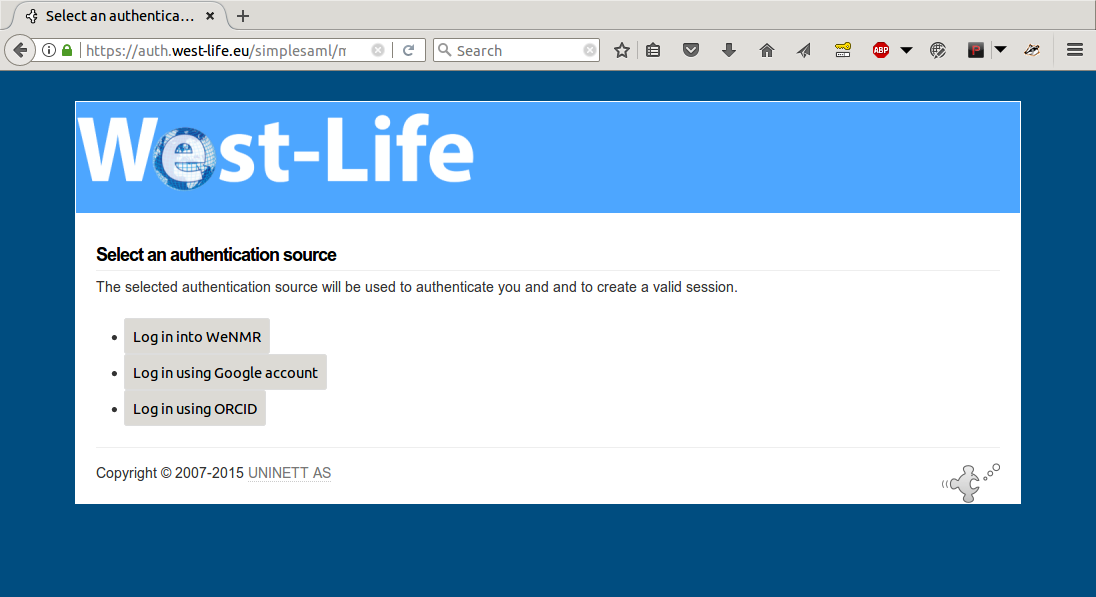
\includegraphics[width=.9\hsize]{westlife-proxy}
\end{center}
\end{frame}




\begin{frame}{Security Assignment \#2}
\begin{itemize}
\item Enable SAML on the portal and link it with the West-Life IdP-SP Proxy
\end{itemize}

\nadpis{Actions to perform}
\begin{itemize}
\item Start with \code{saml\_setup.sh}
\item Extend saxsPortal to run the script
\item After the portal is deployed perform additional steps:
\begin{itemize}
\item Send SP metadata to IdP
\begin{itemize}
  \item You can find metadata of your SP at \code{https://\$HOSTNAME/mellon/metadata}
  \item Check that the link is correct, and let us know
\end{itemize}
\item Verify the authentication after the SP has been registered
\begin{itemize}
  \item Visit \code{https://\$HOSTNAME/auth\_test/}
  \item You should be redirected to IdP (\code{auth.west-life.eu})
  \item Use your credentials to log in
  \item You should be redirected back to SP and see an environment dump
\end{itemize}

\end{itemize}
\end{itemize}

\end{frame}


\begin{frame}{Access Control based on Attributes}
\begin{itemize}
\item IdP release two pieces of information
\begin{itemize}
\item Information about successful authentication
\item Additional attributes linked to the user
\end{itemize}

\item Attributes provides further information, like name, email attributes,
affiliation, \ldots
\item Attributes issued by a Proxy may also carry VO specific information (group membership,
etc.)
\item Few catches though
\begin{itemize}
\item Attribute release policy -- improved lately
\item Different naming and/or semantics of attribute release by different
IdP
\end{itemize}

\item Utilization of attributes for access control
\begin{itemize}
\item Access rules enforced by web server
\item Access control implemented by the application (e.g. mapping to
internal identities).
\end{itemize}

\end{itemize}

\end{frame}

\begin{frame}{Security Assignment \#2}
\begin{itemize}
\item Take a look at the application and try use attributes returned by the
IdP
\item Consult \code{https://\$HOSTNAME/auth\_test/} to see what attributes
are returned by the IdP
\end{itemize}
\end{frame}


\end{document}
